%!TEX root = ../dissertation.tex

\chapter{Evaluation}
\label{chapter:evaluation}

In this Section we measure and profile the resources required for the system operation in order to discover if our choice of protocols and mitigation strategies is suitable for \gls{IoT} hardware. 
This ranges from the memory required for the nodes operating system and protocol stack, to the hardware power consumptions. 
Furthermore we evaluate our bootstrapping infrastructure by measuring the time required for uploading a firmware to the new device and the ease of use by counting the steps required for the process to take place. 
Each following subsection both presents the collected data and explains the process and technologies involved in obtaining it.

\section{Hardware Suitability}
In order to evaluate if the \gls{IoT} hardware is capable of supporting our choice for the stack of protocols security measurements it is necessary to measure the firmware size. 
For that task, the \textit{msp430-size}\footnote{http://www.ti.com/tool/msp430-gcc-opensource} tool was used. 
This tool analyses the firmware file and outputs the amount of \textit{text}, \textit{data} and \textit{bss}.
\textit{Text} corresponds to code and constants, \textit{data} is for initialized variables and \textit{bss} is for uninitialized data (which is initialized with zero in the startup code).
The total amount of flash memory can be calculated from the sum of the text and data parameters.
The total amount of \gls{RAM} memory can be calculated from the sum of the data and bss parameters.
Both the firmware without security mechanisms and the one with link-layer security were analysed for their Flash and RAM usage. 
The results can be found in Table \ref{tab:space_req}. The inclusion of link-layer security software represents a 3.02\% increase in Flash usage and a 1.02\% increase in RAM usage.

\begin{table}
\centering
\caption{Memory Usage}
\label{tab:space_req}
\begin{tabular}{|c|c|c|} \hline
Security Mechanism&Flash(KB)&RAM(KB)\\ \hline
No-Sec& 59.56& 13.54\\ \hline
LLSec& 61.36& 13.80\\ %\hline
%DTLS& 84.38 & 15.66\\ \hline
%LLSec and DTLS& 86.18& 15.91\\
\hline\end{tabular}
\end{table}

In order to be considered an \gls{IoT} capable device for this work, the selected hardware should possess a 802.15.4 radio, be capable of being battery powered and provide development tools like sensors and actuators that would be mapped to the application layer endpoints. 
The board also needs to be compatible with the selected operating system and provide low-power modes of operation. 
With all this in consideration, the Zolertia RE-Mote\footnote{http://zolertia.io/product/hardware/re-mote} board was selected since it fulfilled all the requirements and also provided an integrated cryptoprocessor while maintaining a low-power operation.
On the other hand, to assure our firmware size is a proper fit for current \gls{IoT} hardware we did not not only verify that if fits the Zolertia RE-Mote memory but also compared it to two other boards also designed for \gls{IoT} applications. 
The boards are the Arago Systems Wismote\footnote{http://www.wismote.com} and the Texas Instruments CC2538DK\footnote{http://http://www.ti.com/tool/cc2538dk}. 
The device's memory is shown in Table \ref{tab:hardware_memory} and allows us to conclude that our solution is practical for the target hardware.

\begin{table}
\centering
\caption{Hardware Memory}
\label{tab:hardware_memory}
\begin{tabular}{|c|c|c|} \hline
Device Name&Flash(KB)&RAM(KB)\\ \hline
Zolertia RE-Mote& 512& 32\\ \hline
Arago Systems Wismote& 128& 16\\ \hline
Texas Instruments CC2538DK& 512 & 32\\
\hline\end{tabular}
\end{table}

\section{Power Consumption}
The introduction of security mechanisms in low-power networks is necessary and desirable. However, due to the low-power characteristics of \gls{IoT} sensor and actuator networks, a substantial increase in power consumption can disrupt the network by quickly draining the available resources. 
To this extent, a power consumption analysis was performed on our selected board in order to determine the most suitable battery powering solution following the experimental setup described in Figure \ref{fig:experimental_setup}. 
We performed current measurements during periods of silence as well as during periods of radio activity and calculated the power consumption in Watts(W) from the Power Equation $P = I  V$, where I is the current in Amperes(A) and V is the voltage in Volts(V) as presented in Table \ref{tab:power_consumptions}.

\begin{figure}
  \centering
  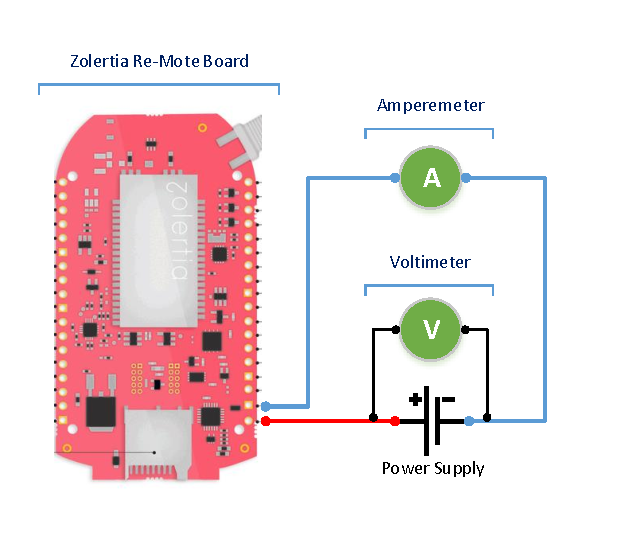
\includegraphics[width=0.65\linewidth]{figures/PowerExperiment.pdf}
  \caption{Power Consumption Experimental Setup}
  \label{fig:experimental_setup}
\end{figure}

\begin{table}
\centering
\caption{Power Consumption}
\label{tab:power_consumptions}
\begin{tabular}{|c|c|c|c|} \hline
Mode&Voltage(V)&Current(mA)&Power(W)\\ \hline
Radio ON& 9.0& 17&0.15\\ \hline
Radio OFF& 9.0& 5.2&0.05\\ 
\hline\end{tabular}
\end{table}

Knowing that the ContikiMAC \gls{RDC} protocol enables the radio to be turned off for roughly 99\% of the time\cite{Dunkels2011}, the collected data shows that our solution maintains the low-power consumptions required for \gls{IoT} environments.

\section{Propagation Delays}
The usage of an Ad-Hoc topology allows to create a network without a pre-existent infrastructure but relies on each participant node to forward data to the other elements of the network. This has impact in the time a message requires to reach its destination based on the number of hops it needs to go through. In order to measure these impacts, a study was conducted where a \gls{CoAP} Client was directly connected to the backend services in a closed room. Additionally, three \gls{CoAP} Servers were providing events to the client, routing data through each other to allow message propagation as depicted in Figure \ref{fig:message_propagation_experiment}. The experiment was conducted with a payload of 180bytes, requiring 3 packets to be sent through the network for each message. Each message was sent ten times from all the three sources. Table \ref{tab:message_propagation_results} presents the results for each server, categorizing each message group by the number of hops required for reaching its destination. The Min-Value represents the fastest message to arrive, the Max-Value represents the slowest message to arrive and the Average-Value the average of the ten attempts conducted for each server. In the case of a packet loss, each server was programmed to resend the packet up to four times, this accounts for the registered Max-Value outliers. In the case of the furtherest away server, where two hops were required for the packet to reach its destination, there were situations were even with four retransmissions the message was never successfully received by the \gls{CoAP} client. It is possible that these failures are caused by the direct exposure of the Wireless Link to a Wi-Fi Access Point located in the corridor. The impact of Wi-Fi networks is well documented in past literature \cite{Dong} and proved to cause interference and even black-out periods. We can conclude that the type of networks being used should preferably be used on locations without heavy Wi-Fi presence, but if that is not possible the network should still perform with high impacts in performance and throughput. 

\begin{figure}
  \centering
  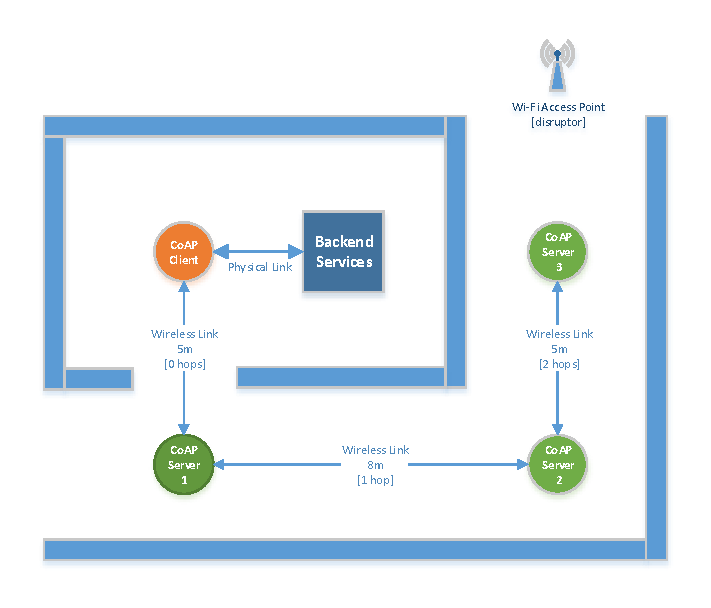
\includegraphics[width=0.8\linewidth]{figures/PropagationExperiment.pdf}
  \caption{Message Propagation Experimental Setup}
  \label{fig:message_propagation_experiment}
\end{figure}

\begin{table}
\centering
\caption{Message Propagation Results}
\label{tab:message_propagation_results}
\begin{tabular}{|c|c|c|c|} \hline
Number of Hops&Min-Value(s)&Max-Value(s)&Average-Value(s)\\ \hline
0& 0.75& 3.47&0.89\\ \hline
1& 1.50& 7.43&2.02\\ \hline
2& 12& N/A&17.9\\ 
\hline\end{tabular}
\end{table}



\section{Bootstrapping Process}
In order to evaluate our bootstrapping process we conducted an experiment on the amount of time (in seconds) required to bootstrap a new node as an indicator of the process efficiency. The process starts with the operator connecting the new device to the bootstrapper and finishes with the operator removing the device from the bootstrapper. During the process the operator needs to open the user interface, select the appropriate device and press the upload button. In the background the system will compile the source code to match the target platform, then it will erase the previous firmware and finally upload the new one. The experiment results are presented in Table \ref{tab:bootstrapping_time}. Although the apparent bootstrapping process time is 34 seconds, the process efficiency is especially important when bootstrapping multiple devices. In this case, after the first one, the user interface and target hardware will already be open and selected and the source code will already be compiled, resulting in a real time of 12 seconds. If needed, an operator could perform up to 300 bootstrapping processes in a single hour, allowing us to conclude that our solution is practical for the presented scenario.

\begin{table}
\centering
\caption{Bootstrapping Timings}
\label{tab:bootstrapping_time}
\begin{tabular}{|c|c|} \hline
Operation&Time(s)\\ \hline
Insert New Device&2\\ \hline
Open User Interface&5\\ \hline
Select Target Hardware&4\\ \hline
Compile Source Code&13\\ \hline
Erase Previous Firmware&5\\ \hline
Upload New Firmware&3\\ \hline
Remove New Device&2\\ 
\hline\end{tabular}
\end{table}

\section{Limitations}
During the development of this solution, and mainly due to compatibility issues, some limitations were raised. The most flagrant is the possibility of compromising a network node and sniffing the contents of the propagated packets. Although we are using \gls{LLSec} and this assures confidentiality, integrity, authenticity of the propagated packets while also providing authentication of the network nodes, in the event of compromising an already deployed node, the messages are cyphered and deciphered on every device, exposing the payload to the attackers. In the future a solution that protects the packets from the source all the way to the destination needs to be addressed so that the solutions can be totality secure against privacy attacks.


